\chapter{振動子、占有数、そして最初の量子場}

量子場の理論は、既知の非重力物理のほぼすべてを扱う枠組みである。この主張は、あらゆる問題が解けるという主張と混同されるべきではない。水素原子は扱いやすいが、ホウ素のような原子に至るまでには計算はすでにはるかに難しくなり、人間は現実的な場の理論計算の及ぶところをはるかに超えている。枠組みが基礎的なものであっても、その方程式を解くことは依然としてきわめて難しい。

したがって、可能な限り初等的な方法で入っていく。この主題は時に\emph{第二量子化}と呼ばれるが、その名は機構を組み立て終えるまでほとんど意味を持たない。最短の道は相対論的な場からではなく、調和振動子から始まる。ばねが要点ではない。重要なのは生成消滅演算子の代数である。その代数を多くのモードについて繰り返せば、生成演算子はもはや単に``振動子を1準位上げる''という意味ではなく、文字通り``粒子を生成する''という意味になる。

\section{代数としての振動子}

1つの振動子について、\(a^\dagger\)を励起を上げるもの、\(a\)を下げるものとする。記法\(a_+\)と\(a_-\)は等価であるが、ダガー記法は場の理論で用いられる言葉を先取りしている。最低状態は
\begin{equation}
a|0\rangle=0,
\end{equation}
を満たし、数演算子は
\begin{equation}
N=a^\dagger a,
\qquad
N|n\rangle=n|n\rangle.
\end{equation}
である。2つの梯子演算子はエルミート共役であり、その本質的な交換子は
\begin{equation}
[a,a^\dagger]=1.
\label{eq:l06-single-commutator}
\end{equation}
である。この小さな代数が振動子のほとんどすべてである。

位置と運動量の適切な線形結合から \(a\) と \(a^\dagger\) を復元できる。正確な規約は \(x\)、\(p\)、\(m\)、\(\omega\) の規格化に依存する。ここで有用な不変な言明は、\(a^\dagger a\) が付加的な基底状態エネルギーを除いて調和振動子のハミルトニアンの二次形式を再構成するということである。したがって
\begin{equation}
H=\hbar\omega\left(N+\frac12\right).
\end{equation}
本稿の議論では定数項を落とし、
\begin{equation}
H=\hbar\omega N.
\label{eq:l06-one-oscillator-hamiltonian}
\end{equation}
で扱う。振動数は一つの励起の代価を教えてくれる。\(n\) を一つ上げるには \(\hbar\omega\) の代価がかかり、\(n\) を一つ下げると同じ量が放出される。

\section{多くの独立な振動子}

次に多くの振動子を取り、それらを\(i\)でラベルする。このラベルは単なる添字であり、虚数単位ではない。モードは有限個かもしれないし無限個かもしれない。独立なばねの集まりは1つの描像を与え、理想的なバイオリン弦の基準モードは別の描像を与える。場の理論への応用では無限個の集まりが重要な場合である。

独立性には演算子としての意味がある。真に独立な部分系に属する演算子は可換である。もし可換でなければ、対応する量を独立に測定することはできず、そもそも系は独立ではない。したがって
\begin{align}
[a_i,a_j]&=0, \\
[a_i^\dagger,a_j^\dagger]&=0, \\
[a_i,a_j^\dagger]&=\delta_{ij}.
\label{eq:l06-many-commutators}
\end{align}
が成り立つ。\(i\ne j\)に対しては、2つのモードに属するすべてのものが可換である。\(i=j\)に対しては、最後の行は式~\eqref{eq:l06-single-commutator}に帰着する。

各振動子はそれぞれ自身の数演算子をもち、一般には自身の振動数をもつ：
\begin{equation}
N_i=a_i^\dagger a_i,
\qquad
H=\sum_i\hbar\omega_i N_i.
\label{eq:l06-many-hamiltonian}
\end{equation}
同時固有状態は完全なリスト
\begin{equation}
|n_1,n_2,n_3,\ldots\rangle,
\qquad n_i=0,1,2,\ldots.
\label{eq:l06-occupation-ket}
\end{equation}
によってラベル付けされる。整数 \(n_i\) は \emph{占有数} と呼ばれ、\(i\) 番目の振動子に対応する。この段階ではそれは単なる用語にすぎない。まもなくそれは一粒子状態を占める粒子を数えることになり、その名は文字通りの意味をもつようになる。

すべての占有数がゼロに等しい状態は
\begin{equation}
|0\rangle\equiv|0,0,0,\ldots\rangle,
\qquad a_i|0\rangle=0\quad\text{for every }i.
\label{eq:l06-oscillator-vacuum}
\end{equation}

\begin{classroomqa}
\lecturetimestamp{00:15:27}
\audiencequestion{振動子の無限族は、バイオリン弦のような系のモードの連続体に対応するのですか。}
\lecturerresponse{はい、理想化された弦においては。実際の弦は原子からできているので、十分に短い波長はやがて微視的なカットオフに遭遇する。それでも連続体模型は、場の理論で用いられるモードの無限個の集まりを動機づける。}
\end{classroomqa}

\section{なぜ梯子の係数は平方根なのか}

\(a^\dagger\)の作用は\(N\)の固有状態を次の固有状態へ上げなければならないが、規格化は係数の余地を残す：
\begin{equation}
a^\dagger|n\rangle=c_n|n+1\rangle.
\label{eq:l06-unknown-coefficient}
\end{equation}

\begin{figure}[htbp]
\centering
\includegraphics[width=0.9\linewidth]{lecture_06_frame_01.png}
\caption{梯子の係数はその規格化が導かれる前に導入される。板書の式は式~\eqref{eq:l06-unknown-coefficient}に再現されている。}
\lectureframe{00:19:38}
\end{figure}

\(c_n\)が実数であるような位相規約を選ぶ。エルミート共役を取ると
\begin{equation}
\langle n|a=c_n\langle n+1|.
\end{equation}
2つの関係を掛け合わせ、規格化された基底状態を用いると、
\begin{align}
c_n^2
&=\langle n|aa^\dagger|n\rangle \\
&=\langle n|(a^\dagger a+1)|n\rangle \\
&=\langle n|(N+1)|n\rangle \\
&=n+1.
\end{align}
したがって、
\begin{equation}
a^\dagger|n\rangle=\sqrt{n+1}\,|n+1\rangle.
\label{eq:l06-raising-rule}
\end{equation}

\begin{classroomqa}
\lecturetimestamp{00:22:35}
\audiencequestion{なぜ\(c_n\)を求める前に\(\langle n+1|n+1\rangle=1\)と置いてよいのか。}
\lecturerresponse{固有ベクトルは最初から規格化された基底として選ばれている。その規格化は\(a^\dagger|n\rangle\)の規格化を決めるものではない。残る情報こそが係数\(c_n\)である。}
\end{classroomqa}

下降規則も同様に従う：
\begin{equation}
a|n\rangle=\sqrt n\,|n-1\rangle.
\label{eq:l06-lowering-rule}
\end{equation}
\(n=0\)では係数が自動的に消えるので、この規則は\(a|0\rangle=0\)を含む。多モードの場合、演算子は自分のスロットの占有数のみを変える：
\begin{align}
a_i^\dagger|n_1,\ldots,n_i,\ldots\rangle
&=\sqrt{n_i+1}\,|n_1,\ldots,n_i+1,\ldots\rangle, \\
a_i|n_1,\ldots,n_i,\ldots\rangle
&=\sqrt{n_i}\,|n_1,\ldots,n_i-1,\ldots\rangle.
\label{eq:l06-multimode-ladders}
\end{align}
他の成分には何も起こらない。

\section{波動関数は量子場ではない}

場を定義する前に、それを馴染み深い波動関数から区別しなければならない。三つの対比がこの移行を整理する。

第一に、一粒子波動関数
\begin{equation}
\psi(x)=\langle x|\psi\rangle
\end{equation}
は状態ベクトルの表現である。それ自体は観測量ではない。我々は位置、運動量、角運動量、その他の演算子を測定する。波動関数は、それらの結果の確率が計算される振幅を与える。

第二に、多粒子波動関数はすべての粒子の位置に依存する。位置ベクトルを暫定的に\(x\)および\(y\)と呼ぶ二粒子に対して、
\begin{equation}
\psi(x,y)=\langle x,y|\psi\rangle.
\end{equation}
ここで\(x\)と\(y\)は二つの異なる粒子を表す。それらは一つの位置ベクトルのデカルト\(x\)成分と\(y\)成分ではない。\(N\)個の粒子では、状態は次で表される：
\begin{equation}
\psi(x_1,x_2,\ldots,x_N).
\end{equation}

第三に、この波動関数は固定された粒子数を記述する。十五粒子波動関数は十五個の位置引数を持ち、十五粒子ヒルベルト空間に属する。それ自体では、粒子数が十五から十四または十六に変わる過程を記述しない。

量子場はこれらの特徴を逆転させる。それは状態ではなく演算子であり、一つの空間点\(x\)に依存し、すべての粒子数セクターを含む状態空間に作用する。``一点''という表現は、一つの自由に変動する位置ベクトルを意味する。\(x\)に一つの数値が割り当てられたという意味ではない。

後に重要となる一つの限定がある。以下で導入される場\(\Psi(x)\)はエルミートではないので、それ自体は厳密な意味での観測量ではない。そのエルミート結合が観測量である。したがって、場は測定可能であるという暫定的な記述は、破棄されるのではなく精密化される。場は演算子値関数であり、そのエルミート結合が測定可能な量を表す。

\begin{classroomqa}
\lecturetimestamp{00:36:52}
\audiencequestion{場が一つの位置の関数であるなら、その位置は変動してよいのか。また、二粒子波動関数の\(y\)はどうなったのか。}
\lecturerresponse{点\(x\)は全空間を変動する。``一つの位置''とは、演算子が一つの空間引数を持つという意味であり、引数が固定されているという意味ではない。\(\psi(x,y)\)において、記号\(x\)と\(y\)は二つの粒子の位置を表す。等価に、それらは\(x_1\)と\(x_2\)である。それらは場の引数の二つのデカルト成分ではない。}
\end{classroomqa}

\begin{classroomqa}
\lecturetimestamp{00:38:15}
\audiencequestion{固定粒子波動関数と場の記述はどのように関係し、それらは異なる種類の粒子を記述しているのか。}
\lecturerresponse{その関連は、これから示す中心的な構成である。粒子は同じ種類である。この講義ではそれらはボソンである。フェルミオンには異なる代数が必要である。}
\end{classroomqa}

\section{箱の中の一粒子}

一時的に通常の一粒子量子力学に戻る。粒子を一次元の箱に入れる。粒子が一つだけなら、ボソンとフェルミオンの区別は無関係である。交換や排他を試す第二の同一粒子が存在しないからである。


\begin{equation}
\psi_1(x),\ \psi_2(x),\ \psi_3(x),\ldots
\end{equation}
をエネルギー固有関数とする。最低モードは壁で消える最も滑らかな波である。次のモードは内部節を一つ持ち、より高エネルギーのモードはより速く振動する。幅\(L\)の理想的な無限井戸では、便利な規格化基底は
\begin{equation}
\psi_i(x)=\sqrt{\frac{2}{L}}\sin\!\left(\frac{i\pi x}{L}\right),
\qquad 0<x<L.
\label{eq:l06-box-basis}
\end{equation}
である。明示的な正弦公式は、定性的な板書スケッチの標準的な実現である。以下の議論は一粒子状態の完全な正規直交系のみを必要とする。

\begin{figure}[htbp]
\centering
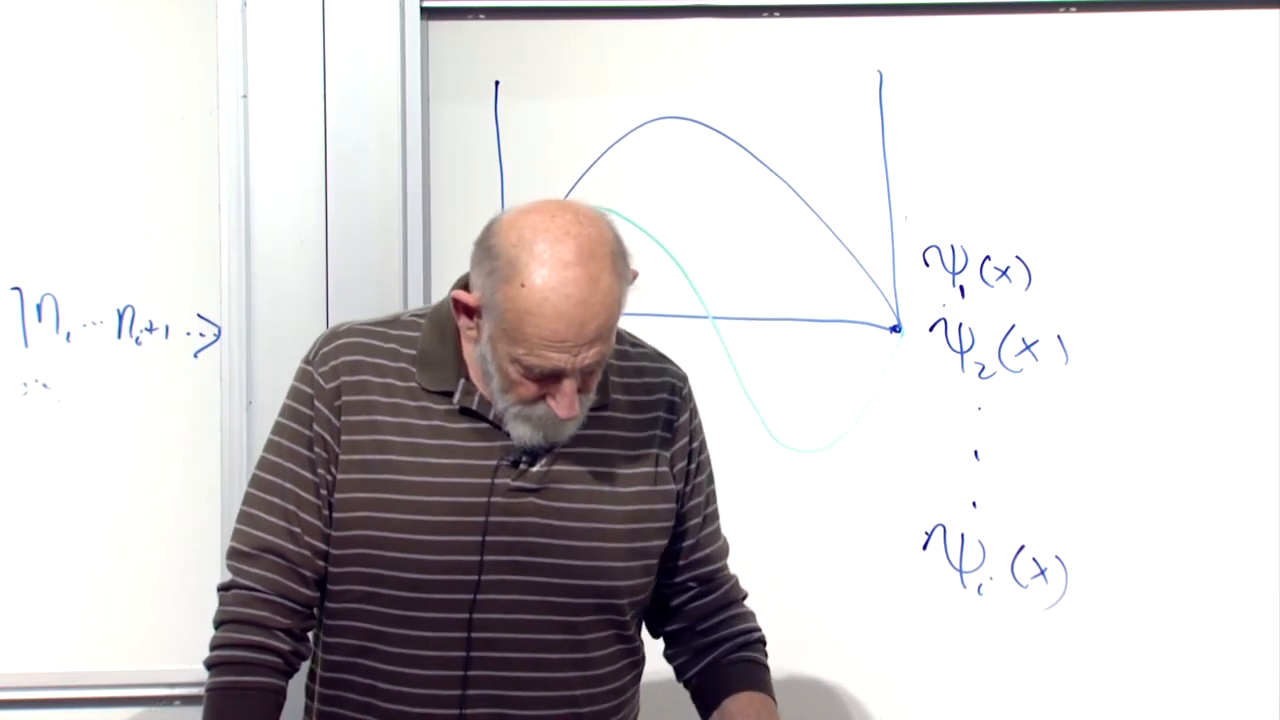
\includegraphics[width=0.9\linewidth]{lecture_06_frame_03.png}
\caption{エネルギー増加順に並べた一粒子箱モード。最初のモードは内部節を持たず、二番目は一つ持ち、省略されたより高次のモードは次第により速く振動する。}
\lectureframe{00:43:10}
\end{figure}

同じ構造は、ライブボードによる遮蔽なしに描き直すことができる。
\begin{figure}[htbp]
\centering
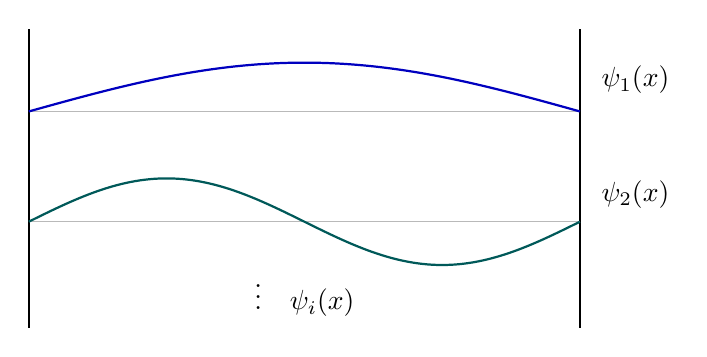
\begin{tikzpicture}[x=1cm,y=1cm]
  \draw[thick] (0,0) -- (0,3.8);
  \draw[thick] (7,0) -- (7,3.8);
  \draw[gray!55] (0,2.75) -- (7,2.75);
  \draw[gray!55] (0,1.35) -- (7,1.35);
  \draw[blue!75!black,thick,domain=0:7,samples=120]
    plot (\x,{2.75+0.62*sin(180*\x/7)});
  \draw[teal!70!black,thick,domain=0:7,samples=120]
    plot (\x,{1.35+0.55*sin(360*\x/7)});
  \node[right] at (7.15,3.15) {$\psi_1(x)$};
  \node[right] at (7.15,1.70) {$\psi_2(x)$};
  \node at (3.5,0.45) {$\vdots\quad \psi_i(x)$};
\end{tikzpicture}
\caption{箱モードの定性的スケッチの明快な再構成。縦方向の変位は読みやすさのために固有関数を分離したものであり、追加の物理的座標ではない。}
\end{figure}

添字\(i\)は一粒子状態を表し、粒子や節の数を表すものではない。箱基底の場合、\(i\)はたまたま内部の節の数より1だけ大きい。各状態はエネルギー\(\varepsilon_i\)をもつ。講義の記法に従えば、このエネルギーを\(\hbar\omega_i\)と書くことができ、\(\hbar=1\)と置けば単に\(\omega_i\)と書ける。

\begin{classroomqa}
\lecturetimestamp{00:39:01}
\audiencequestion{先ほどの独立性の仮定は厳密だったのか、また添字\(i\)は原子中の電子の可能な状態を表しうるのか。}
\lecturerresponse{独立モードの構成では、異なるモード間の交換関係は厳密である。添字は一粒子原子状態を表しうる。しかし粒子が相互作用するならば、単純な独立モードのハミルトニアンはもはや全体像ではない。}
\end{classroomqa}

\begin{classroomqa}
\lecturetimestamp{00:40:34}
\audiencequestion{箱の中の粒子はボソンか。}
\lecturerresponse{ボソンでありうるが、粒子が1個なら統計は問題にならない。排他性と交換は、同一の粒子が複数あるときに初めて意味をもつ。}
\end{classroomqa}

\section{箱モードからフォック空間へ}

ここで、箱の中に任意個の同一ボソンを許す。ある数\(n_1\)が\(\psi_1\)を占め、ある数\(n_2\)が\(\psi_2\)を占め、以下同様である。したがって基底状態は
\begin{equation}
|n_1,n_2,n_3,\ldots\rangle.
\end{equation}
これはすでに多振動子に対して用いた記法そのものである。この同一性は構造的である。すなわち、各一粒子状態に1つの振動子を対応させ、振動子の励起数をその状態を占める粒子数と同一視する。

ここでボソンが本質的であるのは、各\(n_i\)が任意の非負整数でありうるからである。フェルミオンの場合、各一粒子状態は空か単一占有かのいずれかであり、二重占有は決してない。したがって通常の振動子代数をそのまま用いることはできない。

演算子はここで、占有数基底への作用によって定義できる。演算子\(a_i^\dagger\)は一粒子状態\(i\)に1個の粒子を生成し、\(a_i\)は1個を消滅させる。
\begin{align}
a_i^\dagger|n_1,\ldots,n_i,\ldots\rangle
&=\sqrt{n_i+1}\,|n_1,\ldots,n_i+1,\ldots\rangle, \\
a_i|n_1,\ldots,n_i,\ldots\rangle
&=\sqrt{n_i}\,|n_1,\ldots,n_i-1,\ldots\rangle.
\end{align}
これは後付けの類推ではない。この基底上でのボソン生成消滅演算子の定義である。基底が空間を張るため、この定義は線形性によりすべての状態への作用を定める。

\begin{classroomqa}
\lecturetimestamp{00:47:11}
\audiencequestion{\(n_1,n_2,n_3\)は量子状態か。}
\lecturerresponse{ラベル\(1,2,3,\ldots\)は一粒子状態を識別する。記号\(n_1,n_2,n_3,\ldots\)はそれらの状態を占める粒子数である。状態ラベルとその占有数を区別し続けることが、主な記法上の負担である。}
\end{classroomqa}

\subsection{平方根は何をするのか}

因子\(\sqrt{n_i+1}\)は追加の粒子や別個の物理過程を表すものではない。それは演算子に正しい規格化と代数を与える。1モードでは
\begin{align}
a a^\dagger|n\rangle
&=a\bigl(\sqrt{n+1}\,|n+1\rangle\bigr) \\
&=(n+1)|n\rangle,
\end{align}
一方
\begin{equation}
a^\dagger a|n\rangle=n|n\rangle.
\end{equation}
したがってそれらの差は\(|n\rangle\)であり、\([a,a^\dagger]=1\)によって要求される通りである。2つの梯子演算子は、ごく大まかにはそれぞれ\(\sqrt n\)の程度であり、それらの積が\(n\)の程度の数演算子を与えるからである。

\begin{classroomqa}
\lecturetimestamp{00:47:52}
\audiencequestion{平方根因子にはどのような具体的な物理的意味があるのか。}
\lecturerresponse{それは主として数学的な規格化である。それは占有状態が規格化されること、\(a^\dagger a\)が固有値\(n\)をもつこと、そして梯子演算子が振動子の交換関係を満たすことを保証する。ときに数学こそが必要な意味である。}
\end{classroomqa}

\begin{classroomqa}
\lecturetimestamp{00:52:25}
\audiencequestion{生成消滅演算子はその性質と基底への作用によってのみ定義されたのか。}
\lecturerresponse{はい。定義はより原始的な描像から生じる必要はない。その価値は帰結によって試される。完全な基底への作用を定義すれば、演算子は至る所で定義される。そしてこれらの定義は望ましい交換関係を再現する。}
\end{classroomqa}

\begin{classroomqa}
\lecturetimestamp{00:53:22}
\audiencequestion{なぜ\(a_i\)は粒子を別の状態へ移すだけでなく消滅させるのか。}
\lecturerresponse{\(a_i\)は状態\(i\)の占有数を下げるように定義されているからである。有用な問いは、なぜある定義が真であるかではなく、なぜそれが有用であるかである。それが有用なのは、放出と吸収には粒子数を変える演算子が必要だからである。光子は放射が放出されるときに生成され、吸収されるときに消滅する。}
\end{classroomqa}

すべての占有数状態が張る空間は\emph{フォック空間}である。それは真空、すべての一粒子状態、すべての二粒子状態などを、固定された上限なしに含む：
\begin{equation}
\mathcal F=\mathcal H_0\oplus\mathcal H_1\oplus\mathcal H_2\oplus\cdots.
\label{eq:l06-fock-space}
\end{equation}
直和の記法は、通常の\(N\)粒子波動関数が明示しなかったことを明示する。すなわち、すべての粒子数セクターが一つの状態空間に属するのである。

\begin{classroomqa}
\lecturetimestamp{00:54:56}
\audiencequestion{演算子を占有数固有ベクトル上で定義すれば、任意のベクトル上での演算子が決まり、振動子の交換関係もそれに従うのか。}
\lecturerresponse{そのとおりである。占有数ベクトルは基底をなすので、線形性によって定義はフォック空間全体に拡張される。その基底に作用させることでボソンの交換関係が検証される。各一粒子状態は一つの振動子で表され、その振動子の占有数はその状態にある粒子の数である。}
\end{classroomqa}

\subsection{真空と自由ハミルトニアン}

フォック真空は、どの一粒子状態にも粒子が存在しない状態である：
\begin{equation}
|0\rangle=|0,0,0,\ldots\rangle,
\qquad a_i|0\rangle=0.
\end{equation}
ここで\emph{基底状態}という語は誤解を招きうる。最低の\emph{一粒子}状態はモード\(i=1\)である。フォック真空はそのモードにも粒子を持たない。もし粒子が最低モードを占めていれば、\(a_1\)はそれを取り除き、系を真空に戻すことができる。

\begin{classroomqa}
\lecturetimestamp{00:56:19}
\audiencequestion{占有数言語における真空とは何か。最低の一粒子状態は占有されているのか。}
\lecturerresponse{真空ではすべての占有数がゼロに等しく、すべての\(a_i\)によって消滅させられる。最低の一粒子モードは真空では占有されていない。もしそれが占有されていれば、その消滅演算子はその粒子を取り除くことができる。}
\end{classroomqa}

非相互作用粒子では、全エネルギーは加法的である。状態\(i\)にある一粒子がエネルギー\(\hbar\omega_i\)を持つならば、
\begin{align}
H
&=\sum_i \hbar\omega_i N_i \\
&=\sum_i \hbar\omega_i a_i^\dagger a_i.
\label{eq:l06-free-fock-hamiltonian}
\end{align}
二つの等価な読み方がある。それは振動子エネルギーの和であり、一粒子状態ごとに一つの振動子がある。またそれは一粒子エネルギーの和であり、それぞれがそのエネルギーを持つ粒子の数で掛けられている。

場の理論の記法では、\(a_i^\dagger\)は通常生成演算子と呼ばれ、\(a_i\)は消滅演算子と呼ばれる。古い\(a_+\)および\(a_-\)という記法も同じことを言っている。

\section{場が現れる前の明確化}

休憩後のいくつかの質問は、新しい振動子的な帳簿付けを、振動子ポテンシャル中を運動する通常の粒子から区別する。

\begin{classroomqa}
\lecturetimestamp{01:06:09}
\audiencequestion{箱の中の粒子のエネルギー準位は等間隔ではないのに、調和振動子はどこにあるのか。}
\lecturerresponse{一粒子エネルギー\(\omega_i\)は等間隔である必要はない。しかし、各固定モード\(i\)について、そのモードにあるゼロ個、一個、二個、三個の非相互作用粒子のエネルギーは\(0,\omega_i,2\omega_i,3\omega_i\)である。その占有数の梯子が振動子である。それは一つの粒子を調和振動子ポテンシャルに置くこととは異なる。}
\end{classroomqa}

\begin{classroomqa}
\lecturetimestamp{01:08:38}
\audiencequestion{この構成はフーリエ分解と関係があるのか。}
\lecturerresponse{深く関係している。一粒子基底が運動量モードからなるとき、モード関数はサイン、コサイン、または複素指数関数であり、\(a_i\)はフーリエ係数の量子類似物である。一般の基底は三角関数である必要はないが、展開の論理は同じである。}
\end{classroomqa}

\begin{classroomqa}
\lecturetimestamp{01:09:07}
\audiencequestion{すべての粒子に同じエネルギーが割り当てられているのか。また相互作用は含まれているのか。}
\lecturerresponse{同じ一粒子状態を占める粒子は同じエネルギーを持つが、異なる状態にある粒子は一般には同じエネルギーを持たない。今のところ粒子は自由である。すなわち相互作用しない。相互作用があればポテンシャルエネルギーの項が加わるので、ハミルトニアンはもはや式~\eqref{eq:l06-free-fock-hamiltonian}の加法的な和だけではなくなる。}
\end{classroomqa}

\begin{classroomqa}
\lecturetimestamp{01:10:26}
\audiencequestion{各振動子にあった零点エネルギーの半量子はどうなったのか。}
\lecturerresponse{それはハミルトニアンにおける付加的な定数である。定数はすべての演算子と可換であるから、ハイゼンベルクの運動方程式を変えず、通常の非重力測定はエネルギー差に依存する。特別な目的には重要でありうるが、ここで展開している構成には影響しない。}
\end{classroomqa}

自由理論はすでに並外れた力をもつ簿記の道具である。それは多数の粒子だけでなく、状態を変え、現れ、消え、あるいは異なる全粒子数の重ね合わせに存在する粒子をも追跡する。適切なエルミート結合は測定可能であるから、演算子は単なる簿記の記号以上のものであるが、簿記という見方は有用な第一の直観である。

\begin{classroomqa}
\lecturetimestamp{01:14:03}
\audiencequestion{場の理論と量子場の理論は歴史的にどこから来たのか。}
\lecturerresponse{簡潔な歴史的経路は、ファラデーの電場と磁場の物理的描像と、古典場に対するマクスウェル方程式から始まる。プランクは熱放射を研究する中でエネルギー量子を導入し、アインシュタインはその量子化を電磁場そのもの、および光量子と同一視した。その後、ハイゼンベルク、パウリ、とりわけディラックが、1920年代の終わりごろに現代的な演算子の枠組みをまとめるのに寄与した。紫外発散と放射の量子的記述は、決定的な初期の問題の一つであった。これは完全な優先権の割り当てではなく、概略的な歴史である。}
\end{classroomqa}

この歴史的な流れは、なぜ振動子が繰り返し現れるかも説明する。空洞内の古典放射は基準モードに分解される。それらのモードを量子化すると、その励起数が光子数になる。モードを占める数学的な量子は物理的な粒子になる。

\section{ボソン場の演算子}

\(\{\psi_i(x)\}\)を一粒子波動関数の完全正規直交基底とする。
\begin{equation}
\boxed{\Psi(x)=\sum_i a_i\,\psi_i(x)}
\label{eq:l06-field-annihilation}
\end{equation}
を定義し、そのエルミート共役を
\begin{equation}
\boxed{\Psi^\dagger(x)=\sum_i a_i^\dagger\,\psi_i^*(x)}.
\label{eq:l06-field-creation}
\end{equation}
とする。

\begin{figure}[htbp]
\centering
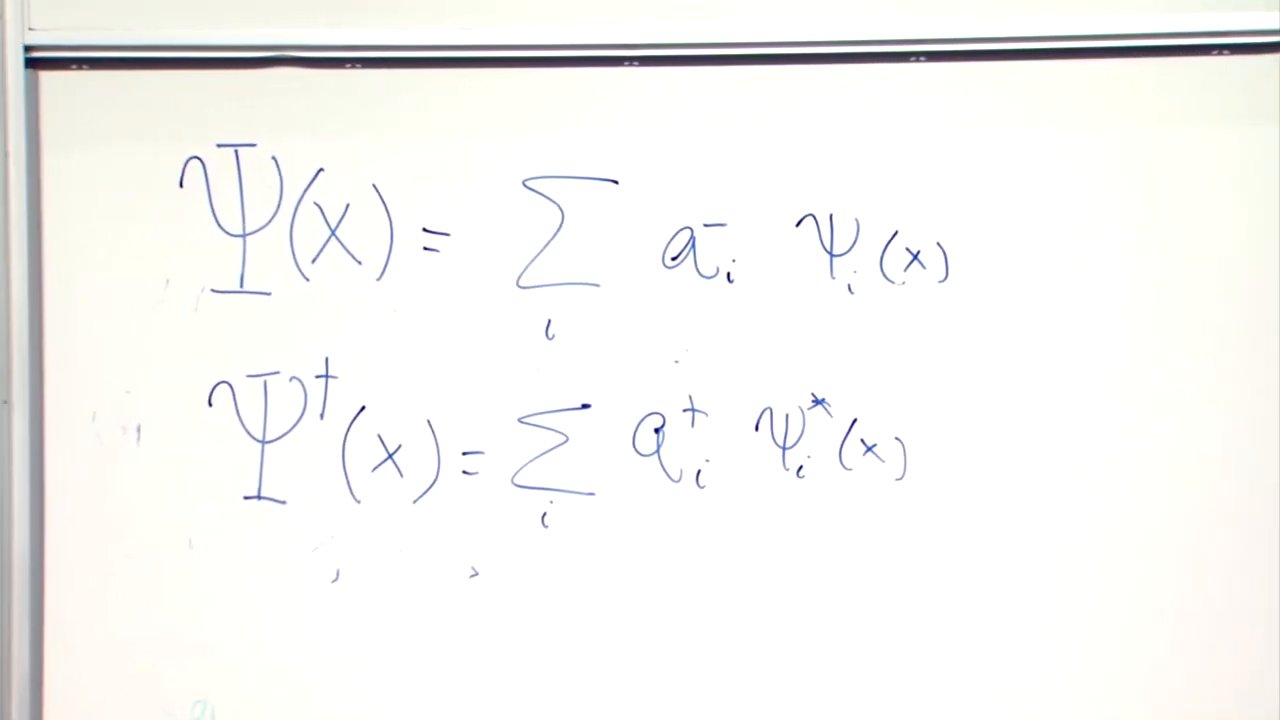
\includegraphics[width=0.9\linewidth]{lecture_06_frame_04.png}
\caption{消滅場とそのエルミート共役の完全なモード展開。式~\eqref{eq:l06-field-annihilation}と\eqref{eq:l06-field-creation}は、組版された形で同じ演算子と複素共役の構造を保っている。}
\lectureframe{01:25:15}
\end{figure}

任意の固定された位置\(x\)に対して、各\(\psi_i(x)\)は通常の複素数である。演算子としての内容はすべて\(a_i\)と\(a_i^\dagger\)にある。\(x\)が変化するにつれて、空間の各点で異なる演算子が得られる。これが、\(\Psi\)が演算子値関数であるという正確な意味である。

基底関数が平面波であれば、式~\eqref{eq:l06-field-annihilation}と\eqref{eq:l06-field-creation}は量子フーリエ展開である。古典的なフーリエ係数が演算子になったのである。箱の中では、基底は代わりに式~\eqref{eq:l06-box-basis}の正弦関数であってもよい。任意の完全正規直交一粒子基底が使える。

\(\Psi\)も\(\Psi^\dagger\)もエルミートではない。観測可能な場は、
\begin{equation}
\Psi(x)+\Psi^\dagger(x),
\qquad
i\bigl(\Psi^\dagger(x)-\Psi(x)\bigr),
\end{equation}
のようなエルミート結合から作ることができ、観測可能な密度は後に\(\Psi^\dagger(x)\Psi(x)\)のような積から作られる。当面の課題は、まず二つの基本的な場が何をするかを理解することである。

\begin{classroomqa}
\lecturetimestamp{01:23:14}
\audiencequestion{右辺のモード関数が通常の波動関数であるのに、なぜ左辺が演算子になりうるのか。}
\lecturerresponse{関数\(\psi_i(x)\)は、\(x\)が選ばれれば数である。因子\(a_i\)は演算子である。数と演算子の積は演算子であり、したがって和も演算子である。\(x\)を変化させると演算子の族全体が得られる。}
\end{classroomqa}

\section{場がすること}

消滅場は真空を直ちに消す。
\begin{equation}
\Psi(x)|0\rangle
=\sum_i\psi_i(x)a_i|0\rangle
=0.
\label{eq:l06-field-kills-vacuum}
\end{equation}
生成場はもっとずっと情報に富むことをする。

\(|i\rangle\)を波動関数
\begin{equation}
\langle x|i\rangle=\psi_i(x).
\end{equation}
をもつ一粒子状態とする。一粒子基底の完全性により
\begin{equation}
\sum_i|i\rangle\langle i|=1.
\label{eq:l06-completeness}
\end{equation}
この恒等式を位置固有状態に適用すると、
\begin{align}
|x\rangle
&=\sum_i|i\rangle\langle i|x\rangle \\
&=\sum_i\psi_i^*(x)|i\rangle.
\label{eq:l06-position-expansion}
\end{align}
フォックの言葉では、一粒子モード状態は
\begin{equation}
|i\rangle=a_i^\dagger|0\rangle.
\end{equation}
である。これを式~\eqref{eq:l06-position-expansion}に代入すると、
\begin{align}
|x\rangle
&=\sum_i\psi_i^*(x)a_i^\dagger|0\rangle \\
&=\Psi^\dagger(x)|0\rangle.
\label{eq:l06-local-creation}
\end{align}
したがって\(\Psi^\dagger(x)\)は\(x\)に局在する粒子を生成し、\(\Psi(x)\)はそこで粒子を一つ取り除く。位置固有状態はデルタ関数的に局在し、一般化された非規格化状態である。物理的に局在した粒子は、規格化可能な波束で場をならすことによって得られる。\editorialnote{講義は理想的な位置固有状態の言葉で話している。波束に関する但し書きは、議論を変えることなく標準的な数学的意味を記録したものである。}

\begin{classroomqa}
\lecturetimestamp{01:36:26}
\audiencequestion{どのような種類の粒子が生成されるかを指定する情報はどこにあるのか。\(x\) における状態はデルタ関数的に局在しているのか。}
\lecturerresponse{各粒子種には別々の場が割り当てられるので、粒子の同一性はどの場が用いられるかによって担われる。引数 \(x\) はそれがどこで生成されるかを指定する。理想的な位置基底では、生成された状態はデルタ関数的局在をもつ。}
\end{classroomqa}

ボソン種の例には光子、重力子、ヒッグス粒子、グルーオンが含まれるが、現実的な場は内部指数も担う。光子でさえ偏極ラベルを必要とする。簡略化されたスカラー場の記法はそれらの余分なラベルを抑制し、生成の原理が見えるようにしている。

\subsection{真空は零ベクトルではない}

方程式
\begin{equation}
\Psi(x)|0\rangle=0
\end{equation}
には、零で表される二つの非常に異なる対象が含まれている。ケット \(|0\rangle\) は真空である。すなわち
\begin{equation}
\langle0|0\rangle=1.
\end{equation}
を満たす規格化された物理的状態である。右辺の結果は零ベクトルである。そのノルムは零であり、規格化できず、物理的状態を表さない。

その違いは加法の下で鮮明になる。零ベクトルを一粒子状態に加えても何も変わらない。真空を一粒子状態に加えると、異なる粒子数セクターの真の重ね合わせが得られる。規格化された係数を用いると、
\begin{equation}
|\chi\rangle=\frac{1}{\sqrt2}\bigl(|0\rangle+|1\rangle\bigr)
\end{equation}
は零粒子と一粒子に対して等しい確率をもつ。これは \(|1\rangle\) と同じではない。

\begin{classroomqa}
\lecturetimestamp{01:37:23}
\audiencequestion{もし \(x\) に粒子が存在しないなら、\(\Psi(x)\) は単に何もしないのか。結果が零になるとはどういう意味か。}
\lecturerresponse{それは元の状態を返すのではない。零ベクトルを返す。真空は空の空間を記述する規格化された状態であり、零ベクトルは長さが零で、いかなる物理的状態も記述しない。零ベクトルに作用する任意の演算子は零ベクトルを返す。}
\end{classroomqa}

\begin{classroomqa}
\lecturetimestamp{01:39:00}
\audiencequestion{零ベクトルではなく真空を一粒子状態に加えるとどうなるか。}
\lecturerresponse{異なる粒子数の振幅をもつ重ね合わせが得られる。対照的に、零ベクトルを加えても一粒子状態は変わらない。\(|0\rangle\) における記号は占有数零を名指すのであり、零ベクトルを意味するのではない。}
\end{classroomqa}

\begin{classroomqa}
\lecturetimestamp{01:41:56}
\audiencequestion{場の展開において、モード関数とその生成演算子または消滅演算子の順序は重要ですか。モード関数は複素数ですか。}
\lecturerresponse{モード関数は通常の数であり、したがってすべての演算子と可換であるから、順序は重要ではない。一般にモード関数は複素数であり得る。選んだ基底が実数か複素数かは、一粒子Schr\"odinger問題に依存する。}
\end{classroomqa}

\subsection{二粒子とボソン対称性の出現}

\(x\) に一粒子を、\(y\) にもう一粒子を生成するには、二度作用させる。
\begin{equation}
|x,y\rangle
=\Psi^\dagger(y)\Psi^\dagger(x)|0\rangle.
\label{eq:l06-two-particle-state}
\end{equation}
点は一致しても異なってもよい。基礎となる生成演算子は可換であるから、
\begin{align}
[\Psi^\dagger(x),\Psi^\dagger(y)]
&=\sum_{i,j}\psi_i^*(x)\psi_j^*(y)
[a_i^\dagger,a_j^\dagger] \\
&=0.
\end{align}
したがって
\begin{equation}
\Psi^\dagger(y)\Psi^\dagger(x)|0\rangle
=\Psi^\dagger(x)\Psi^\dagger(y)|0\rangle.
\label{eq:l06-boson-exchange}
\end{equation}
二粒子の順序を交換しても何も変わらない。これはまさにボソン交換対称性である。したがって我々は振動子代数から出発して、可換な生成演算子から構成される粒子がボソンであることを\emph{導出}できたことになる。フェルミオンには代わりに反可換な演算子が必要となる。

\begin{classroomqa}
\lecturetimestamp{01:42:37}
\audiencequestion{一粒子状態に二つ目の粒子を加えるにはどうすればよいか。}
\lecturerresponse{もう一つの生成場を作用させる。\(y\)に粒子を加えるには、\(\Psi^\dagger(y)\)を\(\Psi^\dagger(x)\)の左側に置いて作用させる。その結果は式~\eqref{eq:l06-two-particle-state}の二粒子状態である。}
\end{classroomqa}

\begin{classroomqa}
\lecturetimestamp{01:46:04}
\audiencequestion{二つの生成場の可換性は、二粒子状態を対称化することと完全に等価か。}
\lecturerresponse{はい。それは \(x\) に一粒子、\(y\) に一粒子をもつ状態を、ラベルを交換して得られる状態と同一にする。これが同一ボソンの定義的な交換性質である。}
\end{classroomqa}

\begin{classroomqa}
\lecturetimestamp{01:46:32}
\audiencequestion{これは \(x\) と \(y\) の粒子が同じ種類のボソンでなければならないことを意味するか。}
\lecturerresponse{はい。引数 \(x\) と \(y\) は位置であり、一方の場は一つの種を記述する。異なる種、および二つの光子偏極のような追加のラベルには、別個の場の成分が必要である。}
\end{classroomqa}

\section{なぜ粒子数が変わりうることが重要か}

もしある問題で粒子の数がいつまでもちょうど37個のままなら、場の言葉は必須ではなく、補助的な記法にすぎない。その真価が現れるのは、粒子が放出・吸収されうるとき、とりわけ粒子数自体が量子変数であるときである。フォック空間では、次の形の状態を扱うことができる。
\begin{equation}
|\Phi\rangle
=c_0|0\rangle+c_1|1\rangle+c_2|2\rangle+\cdots,
\qquad
\sum_{n=0}^{\infty}|c_n|^2=1.
\end{equation}
レーザー場はその重要な例である。一般にそれは、光子数が一つの値に確定した状態ではなく、異なる粒子数の部分空間に属する状態の重ね合わせである。

粒子と場の橋渡しは今や明示的である。モード演算子はエネルギー固有状態における粒子を数え、変化させる。場はそれらの演算子を完全系の波動関数と組み合わせ、指定された位置で粒子を生成または消滅させることができるようにする。調和振動子の代数は、ボソン量子場の初等的言語となった。
